\clearpage

\section{Pulse shaper}

This block applies an electrical filter to the signal. It accepts one input signal that is a sequence of Dirac delta functions and it produces one output signal continuous in time and in amplitude.

\subsection*{Input Parameters}

\begin{itemize}
	\item filterType\{RaisedCosine\} \linebreak
	\item impulseResponseTimeLength\{16\}\linebreak (int) 
	\linebreak (This parameter is given in units of symbol period)
	\item rollOfFactor\{0.9\} \linebreak
	(real $\in$ [0,1])
\end{itemize}

\subsection*{Methods}

PulseShaper(vector$<$Signal *$>$ \&InputSig, vector$<$Signal *$>$ OutputSig) :FIR$\_$Filter(InputSig, OutputSig)\{\};
\bigbreak	
void initialize(void);
\bigbreak	
void setImpulseResponseTimeLength(int impResponseTimeLength)
\bigbreak
int const getImpulseResponseTimeLength(void)
\bigbreak	
void setFilterType(PulseShaperFilter fType)
\bigbreak
PulseShaperFilter const getFilterType(void)
\bigbreak	
void setRollOffFactor(double rOffFactor)
\bigbreak
double const getRollOffFactor()

\subsection*{Functional Description}

The type of filter applied to the signal can be selected trough the input parameter \textit{filterType}. Currently the only available filter is a raised cosine.

The filter's transfer function is defined by the vector \textit{impulseResponse}. The parameter \textit{rollOfFactor} is a characteristic of the filter and is used to define its transfer function.

\subsection*{Input Signals}

\subparagraph*{Number}: 1

\subparagraph*{Type}: Sequence of Dirac Delta functions (ContinuousTimeDiscreteAmplitude)

\subsection*{Output Signals}

\subparagraph*{Number}: 1

\subparagraph*{Type}: Sequence of impulses modulated by the filter (ContinuousTimeContinuousAmplitude)

\subsection*{Example}

\begin{figure}[h]
	\centering
	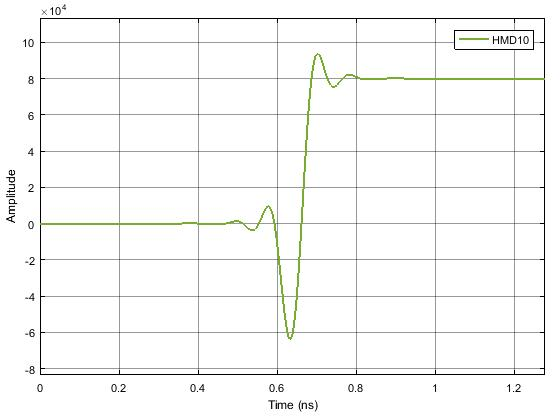
\includegraphics[width=\textwidth]{../homodyne_receiver/figures/PulseShaper_output}
	\label{MQAM6_DeterministicAppendZeros}\caption{Example of a signal generated by this block for the initial binary signal 0100...}
\end{figure}

\subsection*{Sugestions for future improvement}

Include other types of filters.
